
%----------------------------------------------------------------------------
\chapter{Alkalmazás fejlesztése és működése}
%----------------------------------------------------------------------------

\section{Backend}
A backend architekurális felépítéséről a korábbi fejezetben volt szó. 
Most térjünk át az egyes rétegek és egyes funkciók megvalósításának bemutatására.
%----------------------------------------------------------------------------

\subsection{GraphQL Playground}
A legtöbb GraphQL server-hez lehetőségünk nyilik valamilyen interaktív GraphQL szerkesztő felület kiszolgálásra is.
Az alkalmazásban én a GraphQL Playground-ot használtam, a konfigurációt úgy valosítottam meg, hogy éles környezetbe ne szolgálja ki ezt a felületet, csak feljesztői környezet estén.
Ezt környezeti változók segítségével oldaottam meg.

\begin{figure}[!ht]
  \centering
  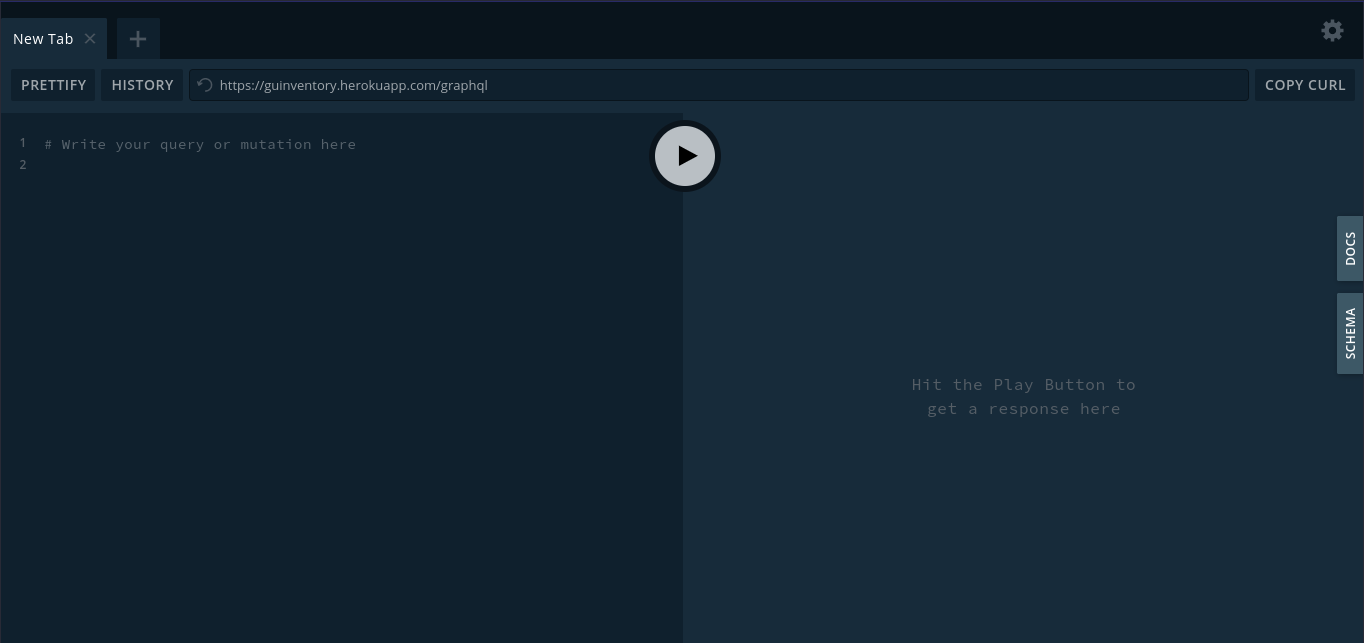
\includegraphics[width=150mm, keepaspectratio]{figures/playground.png}
  \caption{GraphQL Playground}
  \label{fig:playground}
\end{figure}

\begin{figure}[!ht]
  \centering
  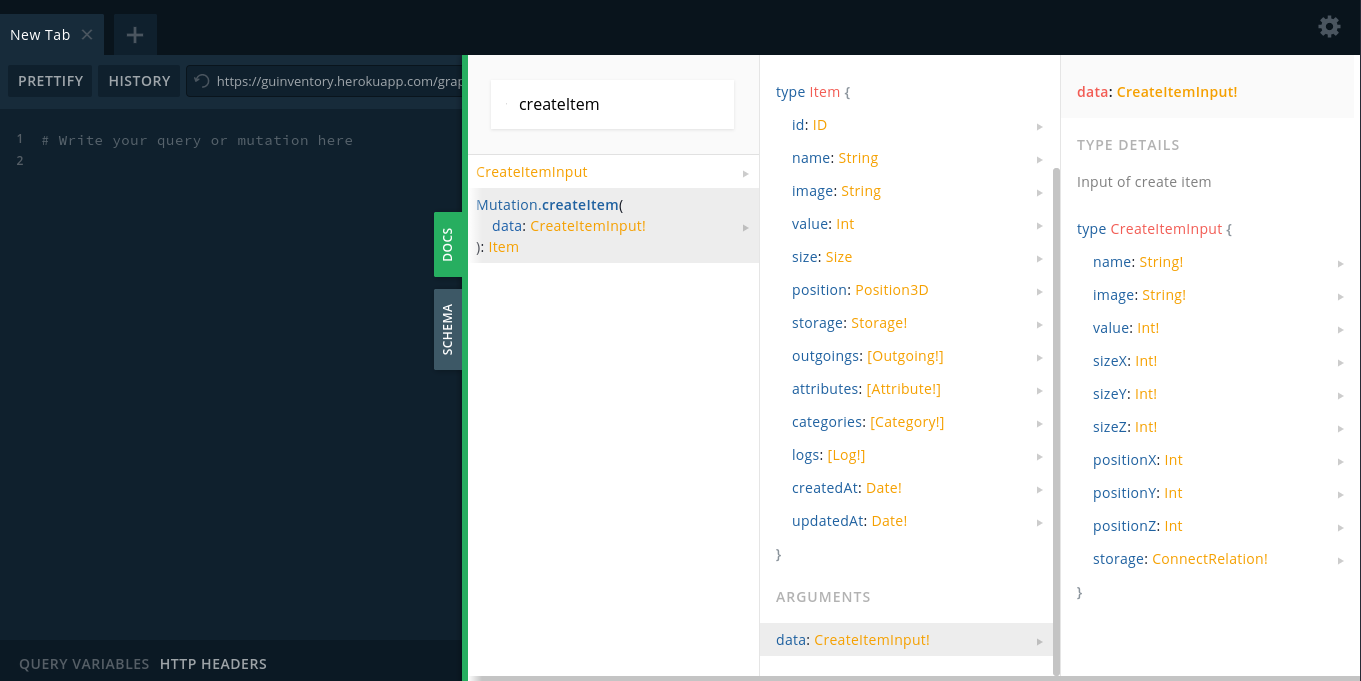
\includegraphics[width=150mm, keepaspectratio]{figures/playground_docs.png}
  \caption{GraphQL Playground Docs}
  \label{fig:playgroundDocs}
\end{figure}
GraphQL Playground es dokumentáció
%----------------------------------------------------------------------------

\subsection{Modellek és kapcsolatok}
Az egyszerűség kedvéért egy az alkalmazásban nem létező modelen mutatom be a működést.

\begin{lstlisting}[style=ES6, caption={Példa model}]
import { objectType } from '@nexus/schema'

export const TypeOfModel = objectType({
  name: 'TypeOfModel',
  definition(t) {
    t.id('id')
    t.string('name')
    t.field('user', {
      type: 'User',
      nullable: false,
    })
  },
})
\end{lstlisting}
%----------------------------------------------------------------------------

\subsection{Resolver felépítése}


\begin{lstlisting}[style=ES6, caption={Eszköz létrehozás resolver}]
t.field('createItem', {
  type: 'Item',
  args: { data: CreateItemInput.asArg({ required: true }) },
  resolve: async (_, { data: { storage, ...rest } }, context: Context) => {
    const item = await context.prisma.item.create({
      data: {
        storage: { connect: storage },
        ...rest,
      },
    })
    await log({
      type: 'CREATE',
      entityId: item.id,
      entityName: 'Item',
      newValues: { storage, ...rest },
      context,
    })
    await publishItemEvent('itemCreated', item, context)
    return item
  },
})
\end{lstlisting}
%----------------------------------------------------------------------------

\subsection{Authentikáció és authorizáció}
GraphQL Shield és JWT

\begin{lstlisting}[style=ES6, caption={GraphQL Shield}]
export const shield = GQLShield(
   {
     Query: {
       warehouses: isGlobalAdmin,
       logs: isGlobalAdmin,
     },
     Mutation: {
       login: allow,
       register: allow,
     },
   },
   {
     allowExternalErrors: true,
     fallbackRule: fallbackRule,
   },
)
\end{lstlisting}

shield szabályok

JWT Ábra, token kezelés, kód magyarázat


%----------------------------------------------------------------------------

\section{Frontend}

%----------------------------------------------------------------------------

\subsection{Útvonalválasztás}
NextJS routing mappa szerkezet lista/kép
\begin{figure}[!ht]
  \centering
  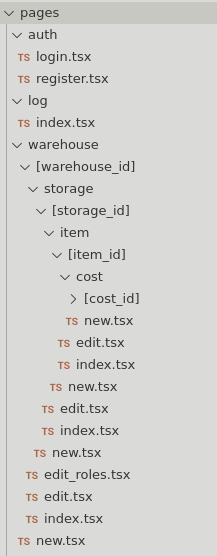
\includegraphics[width=50mm, keepaspectratio]{figures/next_routing.png}
  \caption{Next mappa szerkezeten alapulú routing}
  \label{fig:NextRouting}
\end{figure}

%----------------------------------------------------------------------------

\subsection{Kódgenerálás}
%----------------------------------------------------------------------------

Apollo codegen

hook példa, és használata

\begin{lstlisting}[style=ES6, caption={GraphQL Shield}]
mutation Login($email: String!, $password: String!) {
  login(data: { email: $email, password: $password }) {
    token
  }
}
\end{lstlisting}

\begin{lstlisting}[style=ES6, caption={Bejelentkezés kódrészlet}]
const router = useRouter()
const [login, { loading }] = useLoginMutation()
const toast = useToast()
const { setAuthToken } = useAuthToken()

const onSubmit = async (inputData) => {
  try {
    const {
      data: {
        login: { token },
      },
    } = await login({ variables: inputData })
    setAuthToken(token)
    router.push('/')
  } catch (error) {
    toast({
      title: error.message,
      status: 'error',
      duration: 3000,
      isClosable: true,
    })
  }
}
\end{lstlisting}
%----------------------------------------------------------------------------

\subsection{Validáció}

Yup validációs séma és react form hook

\begin{lstlisting}[style=ES6, caption={Esköz validációs séma}]
import * as yup from 'yup'

export const itemSchema = yup.object().shape({
  name: yup.string().required(),
  image: yup.string().required(),
  value: yup.number().required().typeError('Must be a number'),
  positionX: yup.number().required().typeError('Must be a number'),
  positionY: yup.number().required().typeError('Must be a number'),
  positionZ: yup.number().required().typeError('Must be a number'),
  sizeX: yup.number().required().typeError('Must be a number'),
  sizeY: yup.number().required().typeError('Must be a number'),
  sizeZ: yup.number().required().typeError('Must be a number'),
})
\end{lstlisting}


\begin{lstlisting}[style=ES6, caption={useForm hook}]
const { register, handleSubmit, reset, errors } = useForm<Inputs>({
  resolver: yupResolver(itemSchema),
})
\end{lstlisting}

\begin{lstlisting}[style=ES6, caption={Form}]
<form onSubmit={handleSubmit(onSubmit)}>
  <FormControl mb={4} isInvalid={!!errors.name}>
    <FormLabel htmlFor="name">Name</FormLabel>
    <Input name="name" type="text" ref={register} />
    <FormErrorMessage>{errors.name?.message}</FormErrorMessage>
  </FormControl>
  ...
</form>
\end{lstlisting}

%----------------------------------------------------------------------------

\subsection{Felhasználói felület}
ChakraUI
\begin{figure}[!ht]
  \centering
  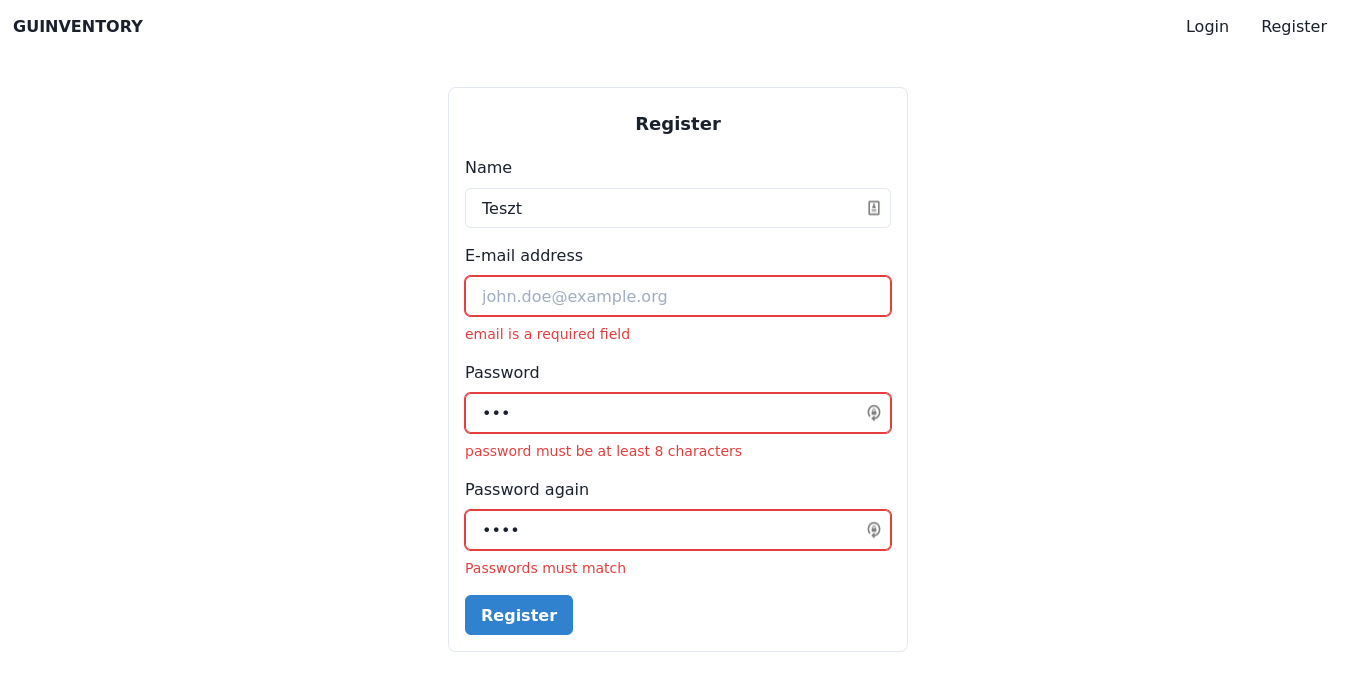
\includegraphics[width=150mm, keepaspectratio]{figures/reg.png}
  \caption{Regisztrációs oldal}
  \label{fig:reg}
\end{figure}

\begin{figure}[!ht]
  \centering
  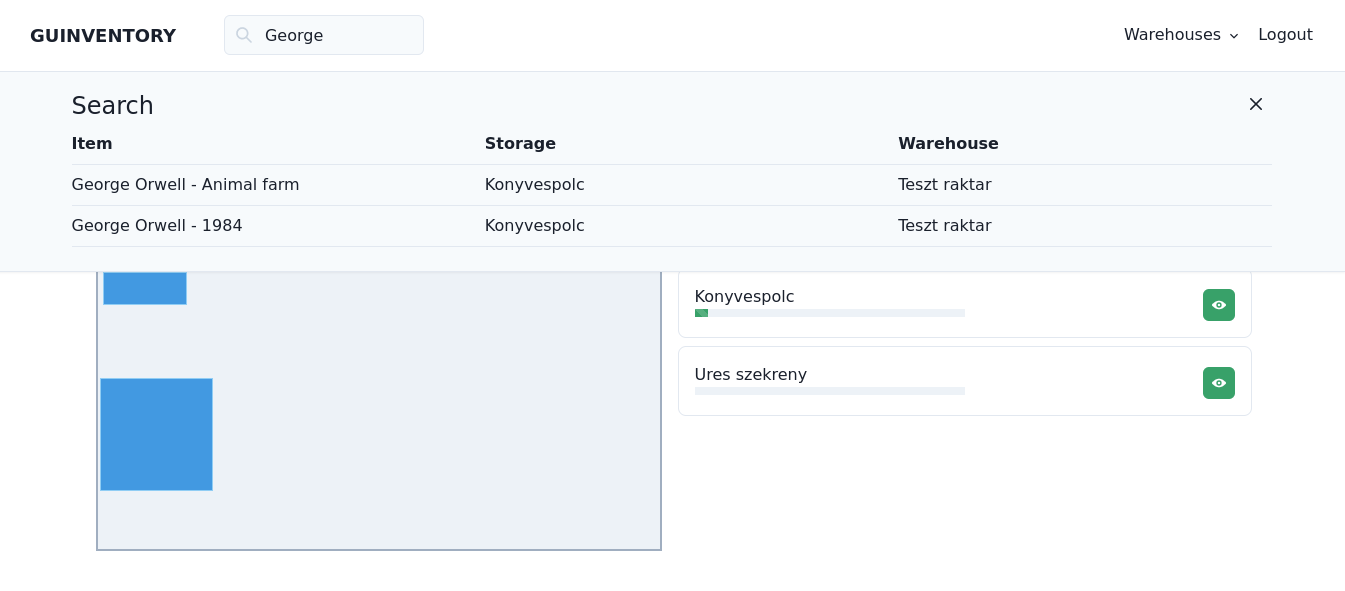
\includegraphics[width=150mm, keepaspectratio]{figures/search.png}
  \caption{Keresés}
  \label{fig:search}
\end{figure}

\begin{figure}[!ht]
  \centering
  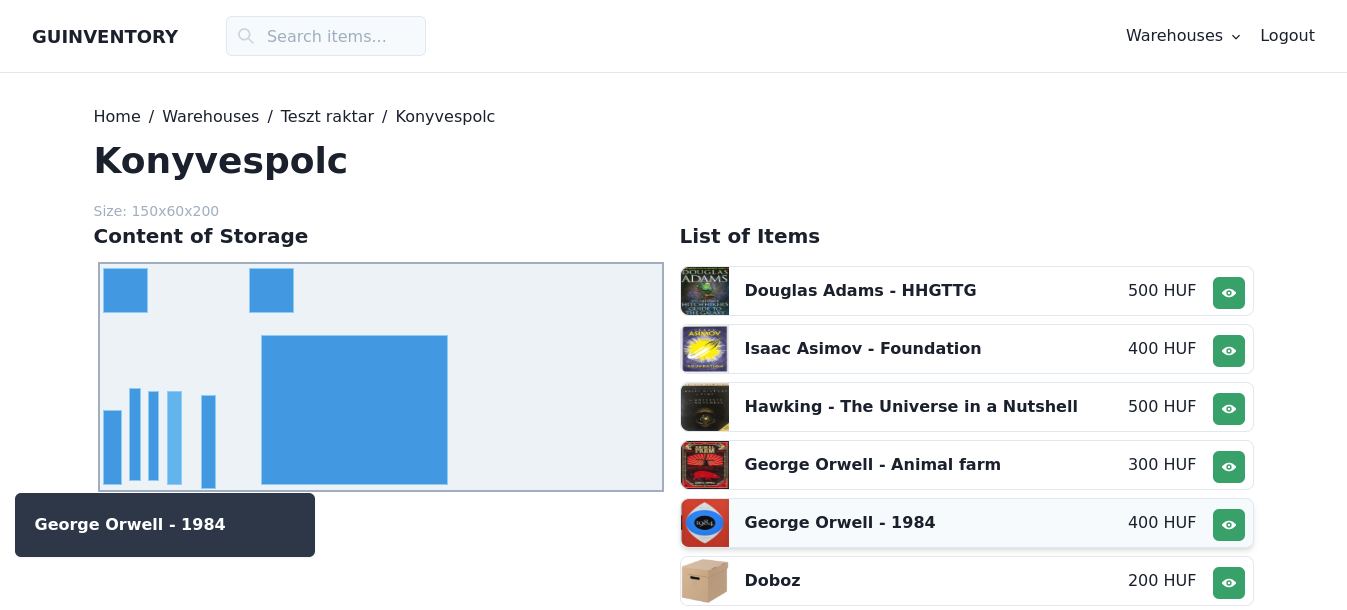
\includegraphics[width=150mm, keepaspectratio]{figures/storage.png}
  \caption{Tároló oldal}
  \label{fig:storage}
\end{figure}

screenshotok az alkalmazásból
példa kód
téma definiálás
dark mode

%----------------------------------------------------------------------------
